\subsection{Vernetzte SBCs}

Abbildung~\ref{fig:arch_03} zeigt die Komponenten der vernetzten SBC-Geräte. Eine Verarbeitungsanwendung kann eine beliebige Anzahl von Prozessoren erhalten, die jeweils ihre Dienste über den ZeroConf / Bonjour-Daemon im Netzwerk anbieten. Der ZeroConf / Bonjour-Daemon wird als Teil des Betriebssystems hier dargestellt. Der ZeroConf / Bonjour-Daemon sendet die Verfügbarkeit, die Verarbeitungsweise und die Portnummern von jedem der verfügbaren Prozessoren.

\begin{figure}[H]
    \centering
    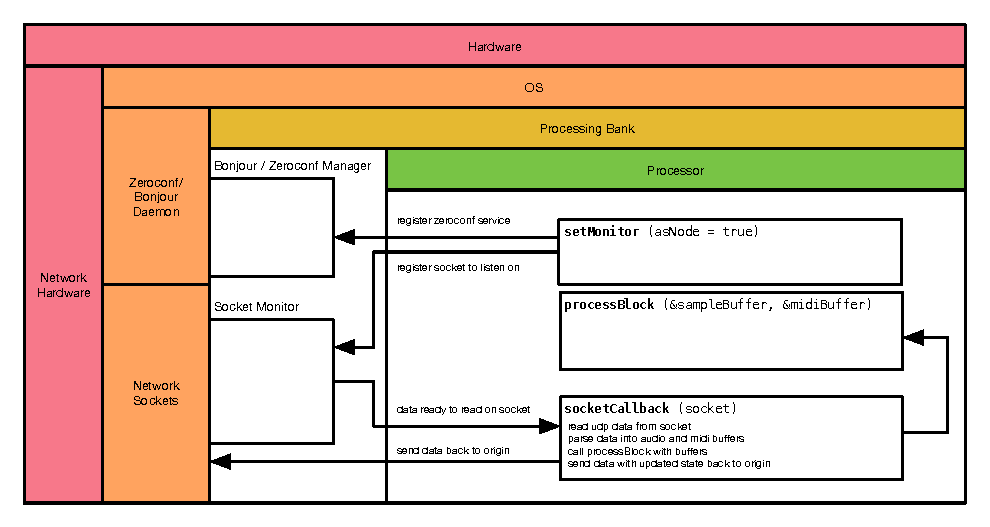
\includegraphics[width=\textwidth]{assets/architecture_03.pdf}
    \caption{SBC-Prozessor-Überblick}
    \label{fig:arch_03}
\end{figure}

Der Prozessor übergibt ein offenes Socket an einen Socket-Monitor und registriert sich als dazugehörendes Socket-Zuhörer-Objekt. Der Socket-Monitor besitzt ein Array von Sockets und einen Verweis auf jeden Zuhörer. Er übt eine „select”-Funktion auf das Array der Sockets aus und wartet. Wenn Daten an einem der Sockets eintreffen, wird die die „select”-Funktion freigegeben, und der Socket-Monitor benachrichtigt die entsprechenden Socket-Zuhörer-Objekte via Rückruffunktion, dass Daten zur Verfügung stehen.

Der entsprechende Prozessor wird über die Rückruffunktion benachrichtigt, liest die Daten, entpackt die Audio-, Zustands- und MIDI-Daten und führt die „processBlock“-Funktion aus. Die Ergebnisse und aktualisierte Zustandsinformation werden dann an den Sender zurückgesandt.

